\documentclass[english,man]{apa6}

\usepackage{amssymb,amsmath}
\usepackage{ifxetex,ifluatex}
\usepackage{fixltx2e} % provides \textsubscript
\ifnum 0\ifxetex 1\fi\ifluatex 1\fi=0 % if pdftex
  \usepackage[T1]{fontenc}
  \usepackage[utf8]{inputenc}
\else % if luatex or xelatex
  \ifxetex
    \usepackage{mathspec}
    \usepackage{xltxtra,xunicode}
  \else
    \usepackage{fontspec}
  \fi
  \defaultfontfeatures{Mapping=tex-text,Scale=MatchLowercase}
  \newcommand{\euro}{€}
\fi
% use upquote if available, for straight quotes in verbatim environments
\IfFileExists{upquote.sty}{\usepackage{upquote}}{}
% use microtype if available
\IfFileExists{microtype.sty}{\usepackage{microtype}}{}

% Table formatting
\usepackage{longtable, booktabs}
\usepackage{lscape}
% \usepackage[counterclockwise]{rotating}   % Landscape page setup for large tables
\usepackage{multirow}		% Table styling
\usepackage{tabularx}		% Control Column width
\usepackage[flushleft]{threeparttable}	% Allows for three part tables with a specified notes section
\usepackage{threeparttablex}            % Lets threeparttable work with longtable

% Create new environments so endfloat can handle them
% \newenvironment{ltable}
%   {\begin{landscape}\begin{center}\begin{threeparttable}}
%   {\end{threeparttable}\end{center}\end{landscape}}

\newenvironment{lltable}
  {\begin{landscape}\begin{center}\begin{ThreePartTable}}
  {\end{ThreePartTable}\end{center}\end{landscape}}

  \usepackage{ifthen} % Only add declarations when endfloat package is loaded
  \ifthenelse{\equal{\string man}{\string man}}{%
   \DeclareDelayedFloatFlavor{ThreePartTable}{table} % Make endfloat play with longtable
   % \DeclareDelayedFloatFlavor{ltable}{table} % Make endfloat play with lscape
   \DeclareDelayedFloatFlavor{lltable}{table} % Make endfloat play with lscape & longtable
  }{}%



% The following enables adjusting longtable caption width to table width
% Solution found at http://golatex.de/longtable-mit-caption-so-breit-wie-die-tabelle-t15767.html
\makeatletter
\newcommand\LastLTentrywidth{1em}
\newlength\longtablewidth
\setlength{\longtablewidth}{1in}
\newcommand\getlongtablewidth{%
 \begingroup
  \ifcsname LT@\roman{LT@tables}\endcsname
  \global\longtablewidth=0pt
  \renewcommand\LT@entry[2]{\global\advance\longtablewidth by ##2\relax\gdef\LastLTentrywidth{##2}}%
  \@nameuse{LT@\roman{LT@tables}}%
  \fi
\endgroup}


  \usepackage{graphicx}
  \makeatletter
  \def\maxwidth{\ifdim\Gin@nat@width>\linewidth\linewidth\else\Gin@nat@width\fi}
  \def\maxheight{\ifdim\Gin@nat@height>\textheight\textheight\else\Gin@nat@height\fi}
  \makeatother
  % Scale images if necessary, so that they will not overflow the page
  % margins by default, and it is still possible to overwrite the defaults
  % using explicit options in \includegraphics[width, height, ...]{}
  \setkeys{Gin}{width=\maxwidth,height=\maxheight,keepaspectratio}
\ifxetex
  \usepackage[setpagesize=false, % page size defined by xetex
              unicode=false, % unicode breaks when used with xetex
              xetex]{hyperref}
\else
  \usepackage[unicode=true]{hyperref}
\fi
\hypersetup{breaklinks=true,
            pdfauthor={},
            pdftitle={Examining play and learning across a year: The PLAY Project},
            colorlinks=true,
            citecolor=blue,
            urlcolor=blue,
            linkcolor=black,
            pdfborder={0 0 0}}
\urlstyle{same}  % don't use monospace font for urls

\setlength{\parindent}{0pt}
%\setlength{\parskip}{0pt plus 0pt minus 0pt}

\setlength{\emergencystretch}{3em}  % prevent overfull lines

\ifxetex
  \usepackage{polyglossia}
  \setmainlanguage{}
\else
  \usepackage[english]{babel}
\fi

% Manuscript styling
\captionsetup{font=singlespacing,justification=justified}
\usepackage{csquotes}
\usepackage{upgreek}

 % Line numbering
  \usepackage{lineno}
  \linenumbers


\usepackage{tikz} % Variable definition to generate author note

% fix for \tightlist problem in pandoc 1.14
\providecommand{\tightlist}{%
  \setlength{\itemsep}{0pt}\setlength{\parskip}{0pt}}

% Essential manuscript parts
  \title{Examining play and learning across a year: The PLAY Project}

  \shorttitle{PLAY Project}


  \author{Rick O. Gilmore\textsuperscript{1,3}, Karen E. Adolph\textsuperscript{2,3}, Catherine L. Tamis-LeMonda\textsuperscript{2}, Kasey Soska\textsuperscript{3}, \& Joy L. Kennedy\textsuperscript{2,3}}

  % \def\affdep{{"", "", "", "", ""}}%
  % \def\affcity{{"", "", "", "", ""}}%

  \affiliation{
    \vspace{0.5cm}
          \textsuperscript{1} The Pennsylvania State University\\
          \textsuperscript{2} New York University\\
          \textsuperscript{3} Databrary.org  }

  \authornote{
    Rick O. Gilmore is in the Department of Psychology, The Pennsylvania
    State University, University Park, PA 16802.
    
    Karen E. Adolph is in\ldots{}
    
    Catherine L. Tamis-LeMonda is in\ldots{}
    
    Kasey Soska is\ldots{}
    
    Joy L. Kennedy is\ldots{}
    
    Correspondence concerning this article should be addressed to Rick O.
    Gilmore, Department of Psychology, University Park, PA 16802. E-mail:
    \href{mailto:rogilmore@psu.edu}{\nolinkurl{rogilmore@psu.edu}}
  }


  \abstract{The overall goal of the PLAY (Play \& Learning Across a Year) project is
to catalyze discovery about behavioral development in infancy. PLAY will
focus on the critical period from 12 to 24 months of age when infants
show remarkable advances in language, object interaction, locomotion,
and emotion regulation. PLAY will leverage the joint expertise of 63
``launch group'' researchers, and capitalize on the Databrary
video-sharing library and Datavyu video-coding tool to exploit the power
of video to reveal the richness and complexity of behavior. Together,
PLAY researchers will collect, transcribe, code, share, and use a video
corpus of infant and mother naturalistic activity in the home to test
behavioral, developmental, and environmental cascades. The project will
demonstrate the value and feasibility of a cross-domain synergistic
approach, and advance new ways to use video as documentation to
facilitate discovery and ensure transparency and reproducibility.}
  \keywords{keywords \\

    \indent Word count: X
  }





\usepackage{amsthm}
\newtheorem{theorem}{Theorem}[section]
\newtheorem{lemma}{Lemma}[section]
\theoremstyle{definition}
\newtheorem{definition}{Definition}[section]
\newtheorem{corollary}{Corollary}[section]
\newtheorem{proposition}{Proposition}[section]
\theoremstyle{definition}
\newtheorem{example}{Example}[section]
\theoremstyle{definition}
\newtheorem{exercise}{Exercise}[section]
\theoremstyle{remark}
\newtheorem*{remark}{Remark}
\newtheorem*{solution}{Solution}
\begin{document}

\maketitle

\setcounter{secnumdepth}{0}



Behavior lies at the heart of developmental science1, and video is a
uniquely powerful tool for capturing the richness and complexity of
behavior2,3. Video documents the microstructure of behavior in real time
and global patterns of change over development4,5---a 12-month-old's
single-word reference to a dog versus a 24-month- old's multi-word
declarative (\enquote{big doggie eat}). Video chronicles who did what,
and how, when, and where they did it6---whether the dog was big, eating,
jumping, or barking, whether the child looked at the dog, touched the
dog, shied away from or approached the dog, and expressed interest,
fear, or joy.

The overarching goal of the PLAY (Play \& Learning Across a Year)
project is to exploit the power of video to catalyze discovery and
transform knowledge about behavioral development in infancy. The project
capitalizes on the NICHD/NSF-funded Databrary video-sharing library7 and
the Datavyu video-coding tool8 developed by PIs Adolph and Gilmore, and
the joint expertise of 63 PLAY \enquote{launch group} researchers in the
United States and Canada (see BIOSKETCHES and LETTERS OF SUPPORT). To do
so, we will create the first, large-scale, sharable and reusable,
transcribed, coded, and curated video corpus of human behavior. And we
will advance new video-based means of documentation to increase
transparency and reproducibility in behavioral science.

We named the project \enquote{PLAY} and use \enquote{unstructured play}
and \enquote{everyday play} to broadly refer to infants' natural
activities while awake. To paraphrase Piaget9, Montessori10, and
Bruner11,12, play is the work of infants. It is an approach to action,
not a particular form of activity. Some of infants' play involves toys
and some play is joyful and goal directed, but all of their spontaneous
vocalizations, interactions with objects and people, and locomotor bouts
involve exploration and opportunities for learning and growth,
regardless of affect or intent.

The project has three aims: 1. To create the first cross-domain,
large-scale, transcribed, coded, and curated video corpus of human
behavior---collected with a common protocol and coded with common
criteria; 2. To answer fundamental questions about behavioral and
developmental cascades; and 3. To demonstrate the scientific value,
feasibility, and scalability of a synergistic approach to collaborative
research, and advance new ways to use video as documentation to ensure
transparency and reproducibility. In this paper, we describe the process
of planning PLAY, our preliminary results from a pilot study, and plans
for a larger scale implementation.

\section{Project Planning}\label{project-planning}

Planning began in late 2015. Adolph, Tamis-LeMonda and Gilmore (PLAY
PIs) invited researchers to join the launch group based on their
interest in open science and infant-mother natural activity in the home,
willingness to collaborate on data collection and coding, lab location,
and domains of expertise (language, gesture, play, object exploration,
tool use, locomotion, posture, physical activity, emotion, temperament,
parent responsiveness, gender, home environment, media use, spatial
demography, and sampling). Nearly every invitee agreed. The launch group
contains 32\% young/new investigators, 66\% women, 19\% non-white, from
varied institutions (public and private universities and colleges,
hospitals, agencies) with varied resources (62\% public universities,
19\% R15-eligible institutions) across the United States and Canada.
Each has committed to produce at least one research study based on the
video corpus.

To distribute the burden of video coding across researchers, the PLAY
PIs recruited 10+ experts for each of four core coding
passes---communication, object interaction, locomotion, and emotion.
These domains represent key areas of development and provide
foundational information when time-locked to video. Compared with other
behaviors (e.g., visual attention), they are quick, easy, and reliable
to code.

Through a yearlong series of telephone conversations with each launch
group member and 12 group webinars, we jointly developed a common
sampling method and protocol (including materials, technical
specifications, questionnaires, and non-video measures), designed common
video codes, and established an infrastructure to divide
responsibilities between PLAY staff and launch group. We achieved
consensus, with input from NICHD program staff, about all aspects of
PLAY at a daylong workshop shared on Databrary56, at NIH in Dec 2016.

The launch group jointly decided that the centerpiece of PLAY would be
900 one-hour videos of infant-mother dyads during natural play in the
home. Home videos are widely believed to be representative of natural
activity, and provide a stark contrast to the 2- to 20-minute
\enquote{snapshots} typical of standard structured lab tasks. Based on
their extensive experience with naturalistic home
observations43,44,46,57-61, launch group members determined that one
hour is sufficiently long to capture an ecologically valid window into
infant and mother natural behaviors. Longer recording times produce
diminishing returns, risk infants becoming excessively tired or hungry,
and increase the cost and burden to families and researchers.

Given the cost of going to families' homes, the launch group also
determined that we should augment natural play with a set of additional
video, questionnaire, and non-video measures, that together would add
only \textasciitilde{}45 minutes to the home visit. This would enable
researchers to test whether variations in natural play, or in
characteristics of distal and proximal environments, predict infant and
mother behaviors when materials and conditions are held constant. Thus,
the solitary and dyadic play tasks are of interest in their own right,
and might also serve as correlates in tests of experiential and
environmental influences.

To obtain objective data on stable home conditions (cracks in walls,
broken windows, ceiling stains, safety issues, etc.), physical layout
(furniture, clutter, space to move, etc.), educational and electronic
media (writing/drawing materials, TVs, computers, etc.), and gendered
characteristics of infants' room, toys, and clothes, we decided to
conduct video home tours. Launch group experts also expressed interest
in understanding whether clothing and footgear affect infants'
locomotion and physical activity, and each takes only moments to video
record. Clothing/footgear videos can reveal gendered features
(bows/frills, superhero emblems, patent leather shoes, army boots)66 and
influences on spontaneous activity and locomotion67. The launch group
also deemed important a variety of questionnaire measures of infant
skills, experiences, and home environment: mothers' report of infants'
vocabulary, locomotor milestones and falls, temperament, and use of
gender labels; mother's report of family demographics, media use,
health, and home chaos; and a researcher-completed survey on physical
characteristics of the home. The PIs developed a custom tablet-based app
to collect these questionnaire data efficiently, limit data input
errors, use a stylus for flexible data entry, and allow automatic
transfer to permanent storage on Databrary. The launch group devised
methods to measure room size with a commercial laser device and ambient
noise level with a commercial decibel meter.

Finally, with input from the launch group, we decided to transcribe all
mother speech and infant vocalizations in formats exportable to CHILDES.
The launch group also developed \enquote{foundational,} time-locked
codes of infant and mother behaviors in four core domains
(communication/gesture, object interaction, locomotion, emotion). These
codes should be informative even to non-experts and are designed to
facilitate further discovery through subsequent coding passes that build
on the prior work. Temporally aligned transcriptions and codes should
enable researchers with expertise in any domain to analyze cascades
within and among these behaviors.

\section{Pilot Study}\label{pilot-study}

Based on the launch group's recommendations, we carried out a pilot
study to test the feasibility of the approach.

\subsection{Methods}\label{methods}

A publicly-accessible wiki \cite{PLAY-wiki} was used to document all
procedures and code definitions. The wiki50 that links descriptions of
every aspect of the protocol with exemplar third-person video clips
(e.g., researcher scheduling home visit). The wiki will also link
descriptions of each code to video clips illustrating the types of
behaviors that do and do not satisfy the coding criteria. These ways of
using video as documentation are innovative, yet simple and inexpensive
to produce, and will serve as a proof of concept for increasing
transparency and reproducibility.

Video as documentation cites

\subsubsection{Participants}\label{participants}

A total of \(n=\) 20 infants were tested, \(n=\) 4 12-month-olds (3
female), \(n=\) 12 18-month-olds (5 female), and \(n=\) 4 (0 female).
All were from the New York City area. Fifteen infants were White, one
was Asian, two reported more than one race, and two did not report a
race. Six were of Hispanic or Latino ethnicity.

\subsubsection{Procedure}\label{procedure}

The PIs designed a wiki50 to aid training, ensure fidelity to the
protocol and codes, and provide complete transparency (Figure 2). The
wiki documents the entire data collection protocol, all video-based
measures including transcription and code definitions, and all
questionnaire and non-video measures. It uses photos and video exemplars
to make text-based descriptions clear and transparent. The wiki makes
cross-site training consistent and cost-efficient and ensure that future
researchers can reproduce our protocol with high fidelity.

The PIs also established that transcription in English or Spanish takes
7-9 hours per hour of video. All four foundational coding passes are
easy to learn (by undergraduate coders on Datavyu) and time efficient
(\textless{} 3 hours for both infant and mother for each coding pass per
hour of video). Note, both infant and mother communicative acts and
gestures together take \textless{} 3 hours to code.

\subsubsection{Data analysis}\label{data-analysis}

For this report, we used R (Version 3.4.4; R Core Team, 2017b) and the
R-packages \emph{acs} (Version 2.1.3; Glenn, 2018), \emph{bindrcpp}
(Version 0.2; Müller, 2016), \emph{choroplethr} (Lamstein, 2017; Version
3.6.1; Lamstein \& Johnson, 2017), \emph{choroplethrMaps} (Version
1.0.1; Lamstein, 2017), \emph{dplyr} (Version 0.7.4; Wickham \&
Francois, 2016), \emph{forcats} (Version 0.3.0; Wickham, 2018a),
\emph{foreign} (Version 0.8.69; R Core Team, 2017a), \emph{Formula}
(Version 1.2.2; Zeileis \& Croissant, 2010), \emph{ggplot2} (Version
2.2.1; Wickham, 2009), \emph{gmodels} (Version 2.16.2; Warnes et al.,
2015), \emph{googlesheets} (Version 0.2.2; Bryan \& Zhao, 2017),
\emph{Hmisc} (Version 4.1.1; Harrell Jr, Charles Dupont, \& others.,
2017), \emph{httr} (Version 1.3.1; Wickham, 2017a), \emph{jsonlite}
(Version 1.5; Ooms, 2014), \emph{lattice} (Version 0.20.35; Sarkar,
2008), \emph{MASS} (Version 7.3.49; Venables \& Ripley, 2002),
\emph{multilevel} (Version 2.6; Bliese, 2016), \emph{nlme} (Version
3.1.131.1; Pinheiro, Bates, DebRoy, Sarkar, \& R Core Team, 2017),
\emph{papaja} (Version 0.1.0.9709; Aust \& Barth, 2017), \emph{plyr}
(Wickham, 2011; Version 1.8.4; Wickham \& Francois, 2016), \emph{psych}
(Version 1.7.8; Revelle, 2017), \emph{purrr} (Version 0.2.4; Henry \&
Wickham, 2017), \emph{readr} (Version 1.1.1; Wickham, Hester, \&
Francois, 2017), \emph{stringr} (Version 1.3.0; Wickham, 2018b),
\emph{survival} (Version 2.41.3; Terry M. Therneau \& Patricia M.
Grambsch, 2000), \emph{tibble} (Version 1.4.2; Wickham, Francois, \&
Müller, 2017), \emph{tidyr} (Version 0.8.0; Wickham, 2017b),
\emph{tidyverse} (Version 1.2.1; Wickham, 2017c), and \emph{XML}
(Version 3.98.1.10; Lang \& CRAN Team, 2018) for all of our statistical
analyses. Datavyu \cite{datavyu} was used for video coding. All code
used in data analysis and for this manuscript may be found in the GitHub
repository associated with the paper \cite{github.paper}.

To compute inter-observer reliability, we ran scripts in Datavyu to
selects a random segment of video (25\% or 5 mins) from each 20- minute
segment of natural play. Inter-observer reliability for the pilot videos
was 96.7\%-99.3\% exact frame agreement (kappas \textgreater{} .93, ps
\textless{} .001) for duration codes (object interactions, locomotion,
emotion) and 94.1\%- 99.5\% code agreement (kappas \textgreater{} .89,
ps \textless{} .001) for categorical events (communicative acts,
gesture).

\subsection{Results}\label{results}

Informal inspection of the videos verified that dyads were unaffected by
the presence of the researcher: After a few minutes of acclimation prior
to natural play, mothers and infants ignore the researcher. Infants cry
and breastfeed; mothers yell, talk on the phone, work on computers, go
about daily chores, change infants' diapers, and give infants snacks.
The PIs verified the efficiency of the new custom tablet app for
collecting questionnaire data. Mothers appeared comfortable with all
procedures, including the video home tour. The PIs found wide variation
in home \enquote{disarray,} suggesting parents present homes as they
would for any other casual visitor. 27 of 28 mothers agreed to share
data. Pilot testing verified the feasibility of collecting all data in
\textless{} 2 hours. So, with 1-2 hours of round-trip travel time, the
entire data collection can be completed in \textless{} 4 hours.

For space reasons, we only summarize here the ambient sound level data
and depictions of the foundational video coding passes.

\subsubsection{Ambient sound levels}\label{ambient-sound-levels}

\subsubsection{Video coding}\label{video-coding}

\subsection{Discussion}\label{discussion}

The pilot study verified that the protocol met the launch group's
criteria on scientific and practical grounds. So we proceeded to design
and plan a full-scale implementation.

\section{Proposed study}\label{proposed-study}

The proposed study builds upon and extends the pilot study.

\subsection{Methods}\label{methods-1}

The same publicly-accessible wiki \cite{PLAY-wiki} will be used to
document all procedures and code definitions.

\subsubsection{Participants}\label{participants-1}

\begin{figure}
\centering
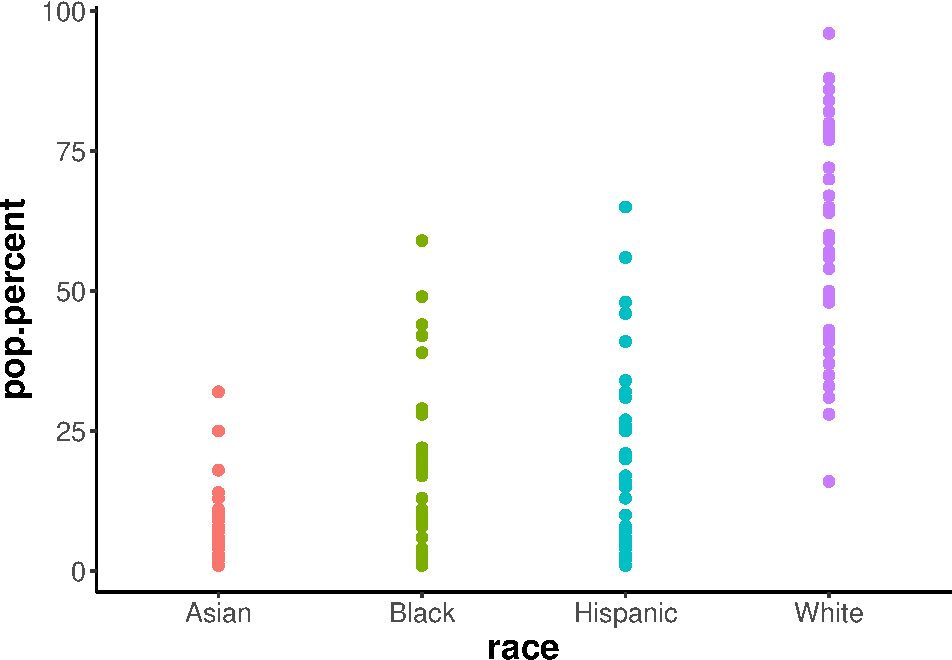
\includegraphics{ibad-ms_files/figure-latex/PLAY-race-plot-1.pdf}
\caption{}
\end{figure}

\begin{figure}
\centering
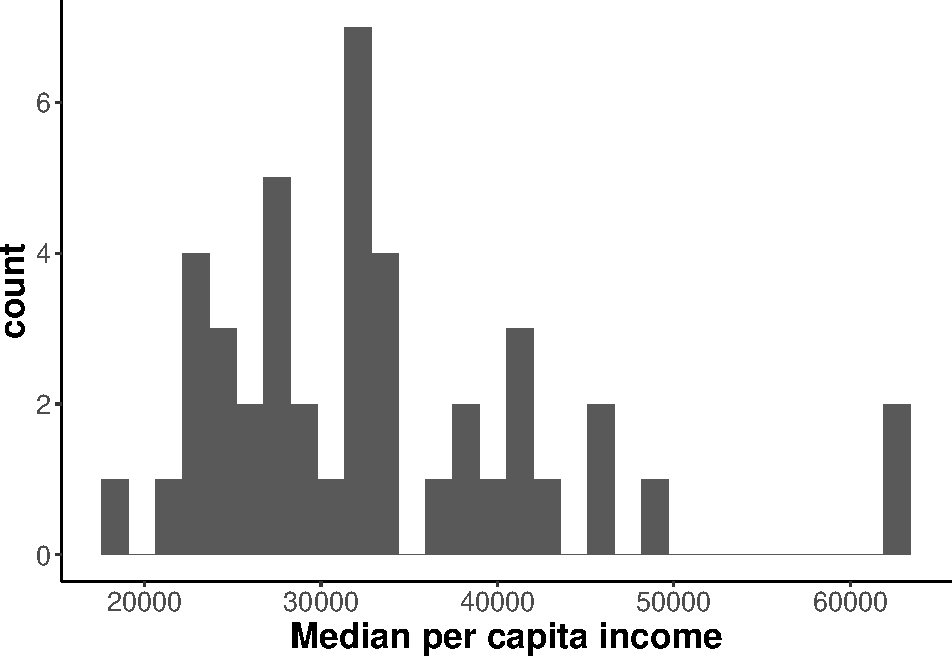
\includegraphics{ibad-ms_files/figure-latex/PLAY-econ-plot-1.pdf}
\caption{}
\end{figure}

We plan to collect data from \(n=900\) infant-mother dyads from 30
different communities in 17 states located around the U.S. Each site
will collect data from 30 infants, 10 each at 12-, 18-, and 24-months of
age (+/- 1 week), with equal numbers of females and males. Figure
\ref{fig:PLAY-sitemap} shows the proposed data collection sites and
non-collecting, data coding and analysis sites.

While not designed to be nationally representative, the data collection
sites are diverse in aggregate, based on Census data.
\ref{fig:PLAY-race-plot} shows the proportion of African American,
Hispanic/Latino, and Asian residents in the counties surrounding the
collection sites from which participating researchers will recruit.
Figure \ref{fig:PLAY-econ-plot} and Figure \ref{fig:PLAY-ed-plot} show
economic and educational attainment indicators. Data collection sites
will have soft, advisory recruiting targets based on these sorts of
measures for their individual communities.

To gather Census data reproducibly, we used the \texttt{chorplethr}
package to download data from the Census Bureau's public API. This
workflow allows us to easily gather and analyze other Census Bureau data
about the communities targeted for sampling.

Families will be two-parent, English and/or Spanish speaking households
with resident fathers, with both parents \textgreater{}18 years old.
Infants will be term firstborns, without birth complications or
disabilities, and 12, 18, or 24 months of age (±1 week); half of infants
at each age and site will be boys. We chose these ages because 12- to
24-months represents a period of important, rapid growth when children
begin talking, using objects in symbolic play, walking, and regulating
emotions. For example, by 12 months, about half of infants can walk and
half still crawl. By 18 months, infants are proficient walkers, and by
24 months, they can run, walk backwards, and walk up stairs16,17. Around
12 months, infants produce their first words. By 18 months, most display
a vocabulary spurt, and by 24 months infants combine words into simple
sentences13,14. But these ages represent only group averages; individual
infants show tremendous variability in these behaviors at each age.

The sample is not intended to be nationally representative. The launch
group deliberated over several sampling strategies27,69,70. Informed by
experts in the launch group, we decided on homogeneous sampling to
contain costs and understand behavioral variation. Homogenous sampling
maintains some control over sample characteristics through a set of
inclusionary criteria (here, firstborn status, English/Spanish home
language, term pregnancy, etc.), while maximizing select aspects of
diversity (e.g., geography, SES) and retaining sufficient power for
group comparisons. We ruled against conventional convenience sampling,
which leaves sampling decisions entirely to researchers' discretion.
Although convenience sampling is easy and cost efficient, it risks
yielding a sample that varies on too many demographic dimensions to
control. At the other extreme, population-based (probability) sampling
is cost-prohibitive due to the required sample size. The sheer volume of
data would prohibit transcription and video coding, and would require
hiring and training special researchers for data collection, rather than
relying on the existing expertise of the launch group.

\subsubsection{Procedure}\label{procedure-1}

During an initial screening call, a researcher will determine
eligibility for participation, and obtain demographic information. The
researcher will schedule a 2-hour visit (weekday or weekend) when
infants are between naps, meals, and baths, and would normally be home
with their mothers. At the end of the visit, the researcher will ask
mothers if the one-hour natural play session was representative of a
typical day at home. If mothers report that infants' behavior or health
was atypical, we will replace the dyad and document the replacement.

The visit will include, in order, parent consent, one-hour natural play,
two structured play tasks, questionnaires, video home tour, and
Databrary sharing permission. Although mothers will agree to share data
in the initial screening call, we will request their signed permission
at the end of the home visit when they are maximally informed. Consent,
sharing permission, and questionnaire data will be entered on the custom
app; paper forms and video camera on tripod will provide backup. Based
on the pilot study, and our own experience in other studies, we
anticipate that most families agree to share data. If families decline
to share, their data can still be stored on Databrary and used by the
collecting researcher for their own purposes.

Natural play: Like the pilot, we will record one hour of infant and
mother activity in the home. Infant and mother will go about their daily
routines without restrictions. They can move from room to room; mother
can do chores; TV, music, or other media can be on. All of these
behaviors were common in our pilot data. The researcher will hand-hold
an HD video camera at the child's eye level, prioritizing view of infant
over mother, keeping the infant's face, hands, and feet in view. If
mother is visible, the researcher will capture as much of her face and
body as possible without losing view of the baby. A cardioid microphone
will amplify infant and mother speech and isolate background noise. Home
visits avoid the artificiality of unfamiliar lab environments,
materials, and tasks, and therefore come closest in fidelity to infant
and mother natural behavior.

We will take several precautions to minimize effects of experimenter and
camera presence on dyads72,73. We will train researchers to remain
unobtrusive. They will stay at a distance, resist talking to mother or
infant, and watch the infant through the viewfinder to avoid eye
contact. Filming will begin after several minutes of infant-mother
acclimation to the camera and researcher.

Solitary play will entail infants playing with a set of 10 nesting cups
(placed half up, half down) while sitting on a mat with mother nearby
but not interacting (2 minutes). Nesting cups can reveal developmental
differences in attention, manual action, spatial problem solving, and
symbolic play. Younger pilot infants manually explored the cups but had
difficulty nesting consecutive sizes; older pilots nested cups and used
them symbolically (e.g., pretended to drink). In dyadic play infant and
mother will play together on the mat with a standard set of toys (3
minutes)--- truck, doll, baby bottle, small blanket, 2 tea cups, plates,
and spoons---with mother instructed to \enquote{share the toys with her
child.} The toys are conducive to non-symbolic (stacking plates, cups),
symbolic (feeding doll, putting doll to sleep), and gendered play (with
truck versus doll).

Following the play episodes, the researcher will walk through each room,
filming walls, floors, ceilings, windows, room contents (including
infants' toys, books, media), and the contents of infants' closets and
drawers. The mother will name each room, describe infant's access to
rooms and spaces, and open closet doors and drawers for filming. Prior
work and piloting ensured that mothers did not find this procedure
intrusive. The researcher will narrate the video with comments about
floor coverings (\enquote{throw rug,} \enquote{linoleum}) and anything
not transparent to video.

During the visit, the researcher will record the clothes (front and
back) and footgear (bottom, side, top) infants wore during the natural
play session, and record the date infants began wearing the shoes and
for how many days/week infants play indoors in shoes, socks, and
barefoot.

After the naturalistic and structured play tasks, the researcher will
interview mothers on a range of infant and family measures that will
yield information about language, locomotion, temperament, gender, home
environment, and health (Table 2). The researcher will administer all
questionnaires orally, and video records the interview (camera on
tripod) for quality assurance, transparency, and possibly later coding.

Language (QL1): We will use the 12-month (words and gestures) and 18- to
24-month (words and sentences) versions of the MacArthur-Bates
Communicative Development Inventory (MCDI). The MCDI is the most widely
used instrument of infant language development, administered to over
60,000 children in 23 languages75. The 12-month MCDI measures receptive
and expressive vocabulary size and communicative gestures; the 18- to
24-month version contains a larger set of vocabulary items and simple
sentence constructions. NL2: Mothers will report the language(s) spoken
to infant by parents and childcare workers. Locomotion (QM1): Mothers
will report the onset ages of hands-knees crawling and walking, using
cell phone videos, photos, and diaries to jog their memories76,77. QM2:
Mothers will report on infants' fall-related injuries. Infant
temperament (QE1) will be indexed with the Rothbart Early Childhood
Behavior Questionnaire (ECBQ), very short form78,79, which measures
dimensions of surgency, negative affect, and effortful control. Gender
(QG1): Mothers will report infants' use of gender labels (e.g., boy,
girl) to refer to themselves or other people. QG2: Mothers will report
their own and the father's attitudes to gender normative behavior (e.g.,
\enquote{I would be upset if my son wanted to dress like a girl}); and
household division of labor (e.g., who does cooking). Environment (NH1):
Ambient noise will be measured during natural play with a decibel meter,
placed in the main room, to record peak and average dB every 100 ms.
NH2: In the home video tour, the researcher will measure room dimensions
with a laser distance measurer. QH3: At the end of the visit, the
researcher will fill out a survey on the home environment (from launch
group member Evans). QH4: Mothers will report use of electronic media
(TV, computers, apps, etc.) by infant and family members (from launch
group member Barr). Health (QF1-4): Mothers will report infant, parent,
and family demographics, infants' health history (based on a subset of
questions from the ECLS-B 9-month and 2-year interviews), childcare
experience, and parents' and family health history including SLI, ASD,
and mental illnesses.

\subsubsection{Video coding}\label{video-coding-1}

Transcriptions and four core coding passes will be scored for both
infant and mother. PLAY staff will transcribe speech at the utterance
level, using standard criteria for segmenting speech74. Utterances will
be defined by independent clauses (statements with subject and
predicate) with modifiers. Intonation and pauses can also define breaks
(e.g., \enquote{You like that . Right?} is two utterances). Mothers'
language-like sounds are typed out phonetically. Infant babbles are
marked with \enquote{b} and non-linguistic vocalizations (cry, laugh,
grunt) with \enquote{c.} Unintelligible utterances are marked
\enquote{xxx.} Utterances will be time-locked to video, revealing
overlaps in infant-mother speech, and co-occurrence and sequencing of
speech with object interactions, emotions, and locomotion. Spanish
transcriptions will follow the same rules.

Based on transcripts, mothers' utterances will be coded as declaratives
(labels and descriptions of objects and events \enquote{Red};
\enquote{Puppy}), attention-imperatives that solicit infant attention
(\enquote{Look at that}), action-imperatives that solicit infant action
(\enquote{Put it there}), or prohibition-imperatives (\enquote{Stop
it!}); interrogatives (open- and close-ended questions, \enquote{Is it
hot?} with the exception of \enquote{tag} questions, which will be coded
as declaratives, \enquote{That's a ball, right?});
affirmation/conversational fillers (\enquote{Yes!}; \enquote{What's
next?}), and unintelligible. Infants' vocalizations will be categorized
as language (sentences or words), prelinguistic vocalizations (babbling
or vowels), non-linguistic vocalizations (e.g., cry, laugh, scream,
grunt), or unintelligible.

Gestures will be categorized as points, show/hold up (deictic),
conventional (wave bye-bye, thumbs-up), and representational (flapping
arms to represent a bird).

Object interactions will be coded for onset and offset of manual
engagement (touching, manipulating, carrying) with any manipulable,
moveable object or part of an object that moves through space.
Locomotion will be coded for onset and offset of self-generated
locomotion of any form (e.g., crawling, walking, climbing, stepping in
place). Coders also score falls, and periods when the infant is held or
constrained by furniture (e.g., highchair). Emotion will be coded for
onset and offset of positive (smiling, laughing) and negative (crying,
frowning, fussing) facial expressions. Inter-observer reliability:

To verify inter-observer reliability, PLAY staff will rescore 25\% of
each infant's natural play video (5 minutes randomly drawn from each
20-minute segment), blind to the original coders' output (categorical
measures: kappas \textgreater{}.85; duration measures: \% exact frame
agreement \textgreater{} 90\%). If codes are not reliable, PLAY staff
will reassign the videos to a new lab.

\subsubsection{Data analysis}\label{data-analysis-1}

The launch group will jointly establish best practices for PLAY
analyses. Our guidelines will include: recommendations to pre-register
predictions and analyses; the use of procedures that use one portion of
the data set to explore correlations among variables and a separate
subsample to confirm it; the use of reproducible and transparent
workflows for data processing and analyses (e.g., Ruby scripts in
Datavyu; syntax instead of menu-driven commands for SPSS users; scripts
and functions for R users); a commitment to openly sharing supplementary
video codes and operational definitions to avoid unnecessary duplication
of coding efforts; and open sharing of null results as well as positive
findings. We will create means for communication (e.g., a Google group)
among launch group members who wish to discuss, propose, and organize
team efforts focused on answering specific video-based research
questions. In addition, we intend to report how we determined our sample
size, all data exclusions (if any), all manipulations, and all measures
in the study.

\section{General Discussion}\label{general-discussion}

The PLAY corpus will be a treasure trove of data, and it will all be
made available openly to the research community at the end of the study.
Our hope is that it will seed substantial new scholarship.

Researchers can examine real-time behavioral cascades among infant
behaviors, among mother behaviors, and between infants and mothers. They
can test whether particular infant behaviors are temporally connected
(e.g., vocalizations and gestures) or independent (vocalizations and
locomotion). They can test infant-to-mother cascades and vice versa,
such as whether infant emotional expressions affect real-time language
input from mother. Prior correlational work, for example, shows that
infants who express higher quantities of negative emotions display lower
levels of language development on the MCDI and later language
milestones37,80. But the evidence for these findings offers limited
insight into the real-time behaviors that underlie the correlations81.
With PLAY, researchers can examine real-time behavioral cascades by
testing whether infants' negative emotions (Table 1 VE1) hinder
interactions with objects (Table 1 VO1) and/or vocal and gestural
communications (Table 1 VL2-3), and consequently, lead to low quantity
and diversity of mother speech (Table 1 VL1-2). Infant emotions could
also facilitate language learning: Emotional expressions might elicit
mental state terms and emotion words from mothers (e.g., \enquote{You
think mommy's leaving?}, \enquote{Why are you sad?}). Regardless,
whether and how infant emotions affect their language development
requires data on the words mothers use preceding, during, and following
infant emotional behaviors in real time.

PLAY's three age groups and measures of skill and experience (e.g.,
MCDI, walking experience) allow researchers to investigate developmental
cascades in new ways. We can examine age-related changes in temporal
coordination among infant, mother, and infant-mother behaviors---such as
whether infants of different ages with different skills elicit different
behaviors in mothers. For example, object interactions in 12-month-olds,
who are typically at the cusp of conventional word use, might elicit
declaratives from mothers (\enquote{That's a truck!}), whereas object
interactions in 24-month-olds, who typically have substantial expressive
vocabularies, might elicit interrogatives (\enquote{What's that?}).
Alternatively, researchers might compare language cascades in infants of
different ages but with similar skills---whether the vocalizations of
18- versus 24-month-olds matched on MCDI vocabulary size elicit similar
or different language input from mothers. Finally, we might compare
real-time cascades in infants of the same age but with different
skills---such as whether 18-month-olds who use isolated words versus
those who combine words into simple sentences, elicit different language
input from mothers. Comparisons of real-time contingencies by infant age
and skill level provide a unique window into understanding developmental
mechanisms that underpin behavioral change.

Environmental cascades. PLAY's rich array of environmental measures,
ranging from distal macro environmental characteristics (e.g., SES,
geographic region) to proximal environmental features (e.g., clutter and
chaos), will advance understanding of how environmental risks affect
everyday opportunities for learning. Researchers might test proximal
environmental cascades on the quantity and quality of infants' object
interactions and locomotion, for example by coding video home tours
(Table 1 VH1) for object availability and using laser measurements of
room dimensions (Table 2 NH2). We can relate environmental features of
clutter, ambient noise, and so on, to mothers' speech and infants'
language development. Researchers can expand the lens of environmental
influences to consider how distal macro factors, such as family SES and
geo-coded data on neighborhood poverty (Table 2 NH5) relate to proximal
environmental measures---objects and space in the home---and in turn
infant behaviors, mother behaviors, and infant language and skill.

Databrary51, funded by NICHD/NSF, is a digital web-based library for
sharing and reusing research videos, clips, and displays. Researchers
can reuse shared videos to ask questions beyond the scope of the
original study2. They can use shared video clips to learn about
procedures and to illustrate findings and displays for teaching3.
Sharing is easy. To mitigate the onerous task of curating a dataset
after the study is completed, Databrary developed an active curation
system. Researchers can use Databrary as a file manager, lab server, and
secure backup prior to sharing52. When they are ready to share, they
need only click a button. Video contains personally identifiable
information, so sharing poses special ethical issues. Advised by ethics
experts, IRB and grants/contracts administrators, and legal counsel,
Databrary developed a policy framework53,54 for sharing identifiable
data based on obtaining participants' permission to share and
restricting access to authorized researchers under the oversight of
their institutions. Since the Databrary website went live in 2014, 580+
researchers (including the launch group) and 245+ affiliates from 330+
institutions around the world are authorized. The repository contains
7820+ hours of video from 7830+ participants. Datavyu8,55 is a powerful,
flexible, coding tool that allows researchers to manipulate the
temporal-spatial properties of behavior and to tag portions of the video
for events and behaviors of interest. With fingertip control over video
playback, they can run the video forward and backward at varying speeds
(±1/32- 32x normal speed) or jog frame by frame to determine when
behaviors began and ended, freeze frames to dissect behavior into its
component parts, zoom in/out to focus on details or the larger context,
and label behavioral events with categorical and qualitative codes. Each
code is time-locked to the video to facilitate tests of behavioral
cascades and real-time contingencies based on sequential order,
duration, and begin/end times of events. A full scripting language
allows researchers to manipulate the spreadsheet, error-check entries,
import other data streams, and export data to their specifications for
analyses. The latest Datavyu release has new features to reduce the
notoriously high cost of transcribing infant and mother speech in noisy
contexts, time locked to video, at the utterance level (from the typical
10-12 hours per hour of video to 7-9 hours).

Naturally, The creation of a large dataset with many variables raises
the possibility that a particular statistically significant finding may
be spurious. In particular, correlational analyses among non-video
questionnaire data require special protection against spurious findings
because of the large number of easily available measures (Table 2). The
corpus includes a summary score for each infant on each instrument,
subscores for standard scales, and raw data for each item. For example,
researchers will have access to infants' total productive vocabulary on
the MCDI, the number of words produced within specific categories (e.g.,
animal words; action words), and production of each word. Similarly,
researchers will have access to fully processed, ready-to-analyze data
on infant temperament, locomotor experience, infant health,
environmental chaos, media use, family demographics, and so on. Spurious
results and duplication of analyses are especially likely from these
\enquote{low-hanging fruit.}

In contrast to the ready-to-use questionnaire data, analyses of
time-locked video codes raise other analytic issues. Data from the
foundational coding passes will not be \enquote{ready to go.}
Researchers will need to make decisions about how to process the
data---whether to turn categorical codes into frequencies or rates;
whether to convert onset/offset times into average durations, latencies
from one behavior to another, sequences of behavior, or other analytic
constructs. We will encourage individual launch group members to use
their expertise and Datavyu training to mine the video corpus (by
further coding of natural play and coding of structured play sessions
and the home tour). Additional coding passes will be labor intensive,
and duplication of coding effort would waste researchers' time.

Of course, PLAY's homogenous sampling strategy and cross-sectional
design have limitations. Although the sample will not be nationally
representative, it will capture important demographic variations and can
easily grow. With only one session per dyad, we cannot test stability or
predictive validity of behaviors. However, the protocol and codes can be
easily extended to other populations and to longitudinal designs
(several launch group members plan to do this). If labs assigned to data
collection or coding cannot fulfill their tasks, we will replace them.\\
We will monitor ongoing data collections. If the data are too
homogeneous, we will ask some sites to recruit more than their
allotment. If a lab's codes are not reliable, we will reassign the
videos and retrain the coder.

In conclusion, the PLAY project represents an innovative, synergistic,
cross-domain approach to developmental science that will facilitate
scientific discovery, transparency, and reproducibility we hope for
years to come. We will answer fundamental cross-domain questions about
behavioral, environmental, and developmental cascades. We will create
the first, large-scale, sharable, reusable, fully transcribed, coded,
and curated video corpus of human behavior. We will establish video
sharing of procedures, codes, and findings as a new standard in
developmental and behavioral science.

\newpage

\section{References}\label{references}

\setlength{\parindent}{-0.5in} \setlength{\leftskip}{0.5in}

\hypertarget{refs}{}
\hypertarget{ref-R-papaja}{}
Aust, F., \& Barth, M. (2017). \emph{papaja: Create APA manuscripts with
R Markdown}. Retrieved from \url{https://github.com/crsh/papaja}

\hypertarget{ref-R-multilevel}{}
Bliese, P. (2016). \emph{Multilevel: Multilevel functions}. Retrieved
from \url{https://CRAN.R-project.org/package=multilevel}

\hypertarget{ref-R-googlesheets}{}
Bryan, J., \& Zhao, J. (2017). \emph{Googlesheets: Manage google
spreadsheets from r}. Retrieved from
\url{https://CRAN.R-project.org/package=googlesheets}

\hypertarget{ref-R-acs}{}
Glenn, E. H. (2018). \emph{Acs: Download, manipulate, and present
american community survey and decennial data from the us census}.
Retrieved from \url{https://CRAN.R-project.org/package=acs}

\hypertarget{ref-R-Hmisc}{}
Harrell Jr, F. E., Charles Dupont, \& others. (2017). \emph{Hmisc:
Harrell miscellaneous}.

\hypertarget{ref-R-purrr}{}
Henry, L., \& Wickham, H. (2017). \emph{Purrr: Functional programming
tools}. Retrieved from \url{https://CRAN.R-project.org/package=purrr}

\hypertarget{ref-R-choroplethrMaps}{}
Lamstein, A. (2017). \emph{ChoroplethrMaps: Contains maps used by the
'choroplethr' package}. Retrieved from
\url{https://CRAN.R-project.org/package=choroplethrMaps}

\hypertarget{ref-R-choroplethr}{}
Lamstein, A., \& Johnson, B. P. (2017). \emph{Choroplethr: Simplify the
creation of choropleth maps in r}. Retrieved from
\url{https://CRAN.R-project.org/package=choroplethr}

\hypertarget{ref-R-XML}{}
Lang, D. T., \& CRAN Team. (2018). \emph{XML: Tools for parsing and
generating xml within r and s-plus}. Retrieved from
\url{https://CRAN.R-project.org/package=XML}

\hypertarget{ref-R-bindrcpp}{}
Müller, K. (2016). \emph{Bindrcpp: An 'rcpp' interface to active
bindings}. Retrieved from
\url{https://CRAN.R-project.org/package=bindrcpp}

\hypertarget{ref-R-jsonlite}{}
Ooms, J. (2014). The jsonlite package: A practical and consistent
mapping between json data and r objects. \emph{arXiv:1403.2805
{[}Stat.CO{]}}. Retrieved from \url{https://arxiv.org/abs/1403.2805}

\hypertarget{ref-R-nlme}{}
Pinheiro, J., Bates, D., DebRoy, S., Sarkar, D., \& R Core Team. (2017).
\emph{nlme: Linear and nonlinear mixed effects models}. Retrieved from
\url{https://CRAN.R-project.org/package=nlme}

\hypertarget{ref-R-foreign}{}
R Core Team. (2017a). \emph{Foreign: Read data stored by 'minitab', 's',
'sas', 'spss', 'stata', 'systat', 'weka', 'dBase', ...} Retrieved from
\url{https://CRAN.R-project.org/package=foreign}

\hypertarget{ref-R-base}{}
R Core Team. (2017b). \emph{R: A language and environment for
statistical computing}. Vienna, Austria: R Foundation for Statistical
Computing. Retrieved from \url{https://www.R-project.org/}

\hypertarget{ref-R-psych}{}
Revelle, W. (2017). \emph{Psych: Procedures for psychological,
psychometric, and personality research}. Evanston, Illinois:
Northwestern University. Retrieved from
\url{https://CRAN.R-project.org/package=psych}

\hypertarget{ref-R-lattice}{}
Sarkar, D. (2008). \emph{Lattice: Multivariate data visualization with
r}. New York: Springer. Retrieved from
\url{http://lmdvr.r-forge.r-project.org}

\hypertarget{ref-R-survival-book}{}
Terry M. Therneau, \& Patricia M. Grambsch. (2000). \emph{Modeling
survival data: Extending the Cox model}. New York: Springer.

\hypertarget{ref-R-MASS}{}
Venables, W. N., \& Ripley, B. D. (2002). \emph{Modern applied
statistics with s} (Fourth.). New York: Springer. Retrieved from
\url{http://www.stats.ox.ac.uk/pub/MASS4}

\hypertarget{ref-R-gmodels}{}
Warnes, G. R., Bolker, B., Lumley, T., Randall C. Johnson are Copyright
SAIC-Frederick, R. C. J. C. from, Intramural Research Program, I. F. by
the, NIH, \ldots{} Cancer Research under NCI Contract NO1-CO-12400., C.
for. (2015). \emph{Gmodels: Various r programming tools for model
fitting}. Retrieved from
\url{https://CRAN.R-project.org/package=gmodels}

\hypertarget{ref-R-ggplot2}{}
Wickham, H. (2009). \emph{Ggplot2: Elegant graphics for data analysis}.
Springer-Verlag New York. Retrieved from \url{http://ggplot2.org}

\hypertarget{ref-R-plyr}{}
Wickham, H. (2011). The split-apply-combine strategy for data analysis.
\emph{Journal of Statistical Software}, \emph{40}(1), 1--29. Retrieved
from \url{http://www.jstatsoft.org/v40/i01/}

\hypertarget{ref-R-httr}{}
Wickham, H. (2017a). \emph{Httr: Tools for working with urls and http}.
Retrieved from \url{https://CRAN.R-project.org/package=httr}

\hypertarget{ref-R-tidyr}{}
Wickham, H. (2017b). \emph{Tidyr: Easily tidy data with 'spread()' and
'gather()' functions}. Retrieved from
\url{https://CRAN.R-project.org/package=tidyr}

\hypertarget{ref-R-tidyverse}{}
Wickham, H. (2017c). \emph{Tidyverse: Easily install and load
'tidyverse' packages}. Retrieved from
\url{https://CRAN.R-project.org/package=tidyverse}

\hypertarget{ref-R-forcats}{}
Wickham, H. (2018a). \emph{Forcats: Tools for working with categorical
variables (factors)}. Retrieved from
\url{https://CRAN.R-project.org/package=forcats}

\hypertarget{ref-R-stringr}{}
Wickham, H. (2018b). \emph{Stringr: Simple, consistent wrappers for
common string operations}. Retrieved from
\url{https://CRAN.R-project.org/package=stringr}

\hypertarget{ref-R-dplyr}{}
Wickham, H., \& Francois, R. (2016). \emph{Dplyr: A grammar of data
manipulation}. Retrieved from
\url{https://CRAN.R-project.org/package=dplyr}

\hypertarget{ref-R-tibble}{}
Wickham, H., Francois, R., \& Müller, K. (2017). \emph{Tibble: Simple
data frames}. Retrieved from
\url{https://CRAN.R-project.org/package=tibble}

\hypertarget{ref-R-readr}{}
Wickham, H., Hester, J., \& Francois, R. (2017). \emph{Readr: Read
rectangular text data}. Retrieved from
\url{https://CRAN.R-project.org/package=readr}

\hypertarget{ref-R-Formula}{}
Zeileis, A., \& Croissant, Y. (2010). Extended model formulas in R:
Multiple parts and multiple responses. \emph{Journal of Statistical
Software}, \emph{34}(1), 1--13. Retrieved from
\url{http://www.jstatsoft.org/v34/i01/}






\end{document}
